\section{Introduction}

The Rubin Observatory Data Management System, as described in \textit{Juric et al}\cite{2015arXiv151207914J},
is responsible for creating the software, services, and systems that will be used to
produce the observatory's science-ready data products.  Project requirements on DM
products are documented in change-controlled specifications. DM Verification and Validation activities are planned
to guarantee that survey software and infrastructure both fulfill the system requirements and enable the science that
motivates the project.

In line with the verification approach adopted for the Gaia DPAC project, described in in \textit{Comoretto et al}\cite{10.1117/12.926797}, 
we present here the tooling and procedures used at Rubin Observatory for the documentation of verification and
validation activities. Test activities are managed in Jira, where test cases are created and updated, and test results
are reported. This ensures that all elements to be documented are available in one tool, that maintains a history of
the process. The System Engineering model is synced with the Jira test framework, providing a direct link between
tests and requirements. Test documents can therefore be generated programmatically, avoiding typical problems
such as a lack of traceability, misspelling, duplication of content, and misalignment between documents. The
centralized collection of information permits a high level of automation, where the extraction of test documents is
achieved by a continuous integration process. This systematic approach substantially reduces the time required to
produce verification and validation documentation, and its integration with the project's System Engineering model, 
see \textit{Selvy et al}\cite{10.1117/12.2310125}, ensures full traceability to system requirements.


\section{The Verification and Validation Problem}

The main scope of the verification and validation activity is to ensure that all requirements have been properly implemented and verified.
This includes identifying the requirements, the affected components and the verification procedures.

The Data Management requirements are baselined in the \textit{Data Management Requirement Specification}\cite{LSE-61}, also know as DMSR.
The DM requirements are flowed down from the SRD, the \textit{LSST System Science Requirements Document} \cite{LPM-17}. 
Interface requirements between DM and other LSST subsystems also have an impact on Data Management provided components, 
and therefore need to be considered during Verification and Validation. 
The figure \ref{fig:topdoctree} shows the high level requirements documents flow down.

\begin{figure}
\begin{center}
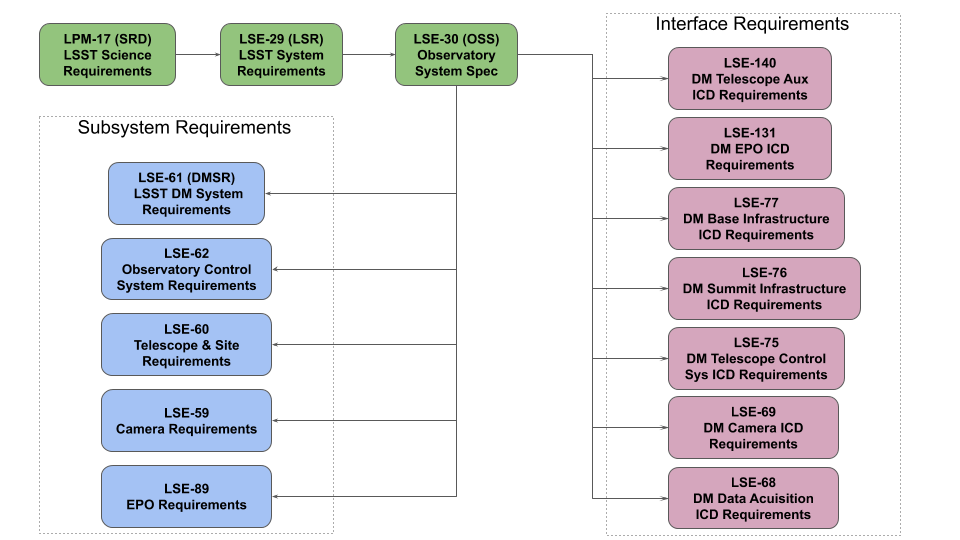
\includegraphics[width=\textwidth]{imgs/TopLevelDocTree.png}
 \caption{The Rubin Observatory top level document tree.}
 \label{fig:topdoctree}
\end{center}
\end{figure}

DM is responsible to fully verify the DMSR requirements and to contribute to the verification and validation of the interface requirements that have an impact on the subsystem.
We guarantee this by creating verification elements associated with each requirement, 4 for the DMSR requirements and 2 for the interface requirements.
Those verification elements are assigned to the validation scientist, 
who will ensure they are properly described and sufficient to fully verify the corresponding requirements. 
The validation scientist will ensure that for each verification element there is at least a test case.
In the case that the provided verification elements are not sufficient, the validation scientist will request more verification elements to be associated with the requirement.
In the opposite case, if a provided verification element is not needed, it will be removed.

The verification activity will be done in order to fulfill test milestones, defined at project level.
For each milestone, a test campaign will be setup. 
Test executions are collected in Jira and coverage information is propagated back to Verification Elements and Requirements.
Test documents, including test reports, are generated automatically from Jira.

\begin{figure}
\begin{center}
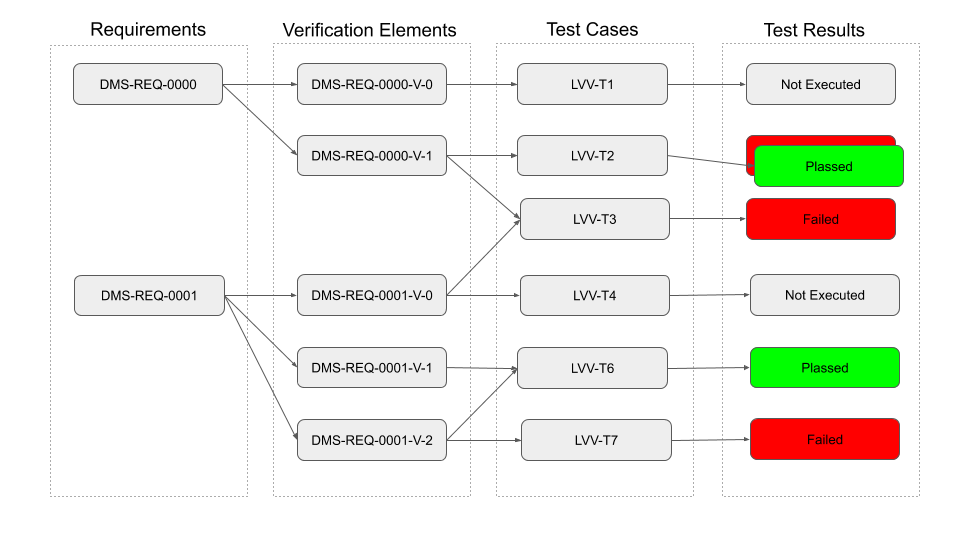
\includegraphics[width=\textwidth]{imgs/VandVSchema.png}
 \caption{Schematic approach to the Verification and Validation.}
 \label{fig:vandvschema}
\end{center}
\end{figure}
% Describe a here a general V&V approach, explain our requirements documents and how they are flowed down from the SRD. DM is responsible to verify requirements that are re

% How do we systematically document the verufication of all the reqirements in this picture in an automated way. 

% GCM to draft a schematic of the approach 
\section{The Verification and Validation Infrastructure}

The verification and validation approach as illustrated in \cite{10.1117/12.2310125}  has been implemented.
Required tools have been put in place, like \textit{Syndeia} and \textit{Docsteady}.


\subsection{Tools}

In this section we give a short description for each tool involved in the Verification and Validation activity.
Figure \ref{fig:vandvtools} gives a schematic overview.

\begin{figure}
\begin{center}
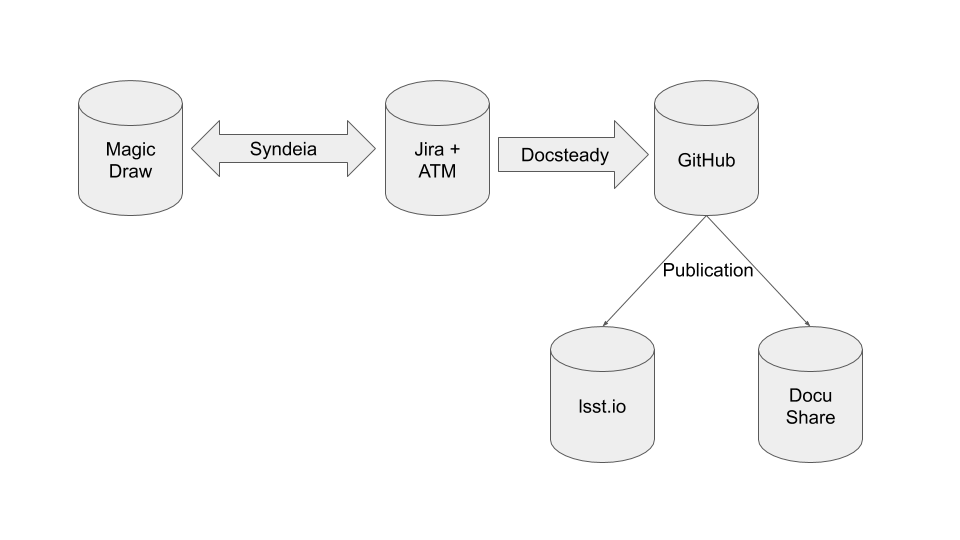
\includegraphics[width=\textwidth]{imgs/VandVtools.png}
 \caption{Schematic overview of the tools involved in the V\&V process.}
 \label{fig:vandvtools}
\end{center}
\end{figure}

\paragraph{MagicDraw}
is the Rubin Observatory Modeling tool. It is used for requirement management. The Verification Elements are created
in MagicDraw and then synchronized to and from Jira using \textbf{Syndeia}. This ensures that the proper 
traceability between requirements and verification elements is in place, and that changes in one part of the system can be propagated through other components.

\paragraph{Jira}
is the Rubin Observatory issue tracking system.
The Adaptavist Test Manager plugin (ATM) provides additional functionalities to Jira to manage test activities.
Jira is hosting all test information, providing to the user an easy-to-use graphic interface.

\paragraph{Syndeia}
is a third party tool that integrates MagicDraw and Jira. First the Verification Elements created in MagicDraw,
are synched in Jira. After the test activity is completed, the information will be synched back to MagicDraw.

\paragraph{Docsteady}
is the tool that permits generation of the test documents, extracting the information from Jira using REST API.
It can be executed manually or automatically, generating the documents in \LaTeX~format.
It can be scheduled on a continuous integration tool like for example Jenkins, making possible that 
the documents are generated continuously.
The extracted documents are managed using Git repositories, and follows the  standard LSST document workflow.
Docsteady is developed internally at LSST and the source code is available at \url{https://github.com/lsst-dm/docsteady}.

\paragraph{GitHub}
is the platform for software version management.
Verification and Validation documents are written in Latex and maintained in git repositories.
Each time a change is made in the document, a new pdf is built automatically in the integrated Travis platform, and made available in the \textbf{lsst.io} landing page.

\paragraph{lsst.io}
is the documentation portal for LSST, see \textit{The LSST the Docs Platform for Continuous Documentation Delivery}\cite{SQR-006}~.
Each document has a lsst.io publication page, where the pdf is pushed by Travis, after each successful build.

\paragraph{Docushare}
is the official Rubin Observatory documentation repository during construction.
Documents are uploaded in Docushare only after their formal approval.


\subsection{Procedures}

The Verification and Validation activities originate from the requirements.
We assume in this document, that the requirements have been properly formalized, documented and approved.
As described early in this paper, a defined number of verification elements is created for each requirement.
When first created, the verification elements have no description. The only information they have is the requirement from where they have been generated.
They are synched to Jira using Syndeia, where the validation scientist ensures that they are properly addressed.

\begin{figure}
\begin{center}
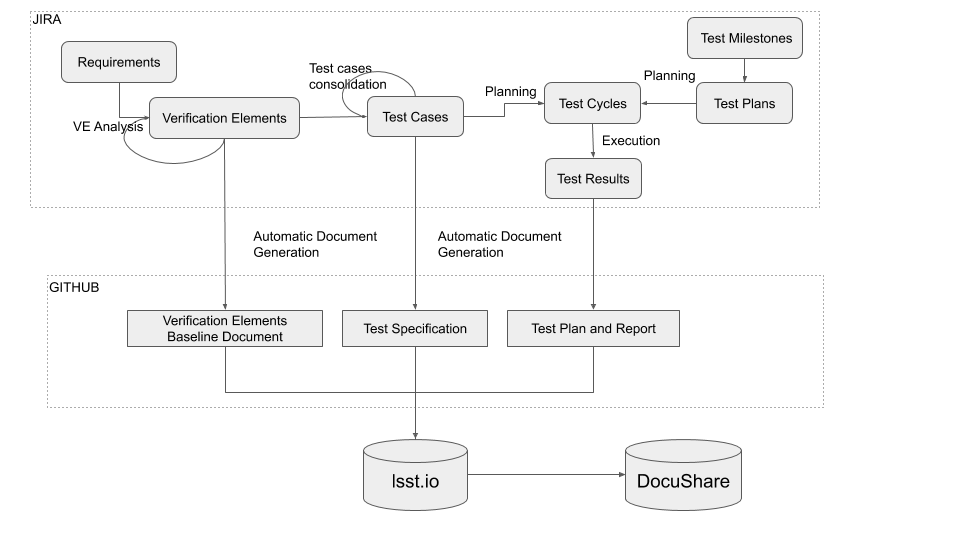
\includegraphics[width=\textwidth]{imgs/VandVprocedure.png}
 \caption{Schematic overview of the V\&V procedure.}
 \label{fig:vandvtools}
\end{center}
\end{figure}


\subsubsection{Verification Elements Analysis}

The first activity, required before starting with any test campaign, is to ensure that each verification elements is cometed with the relevant information.
This is done by the validation scientist, or delegated.

As a result of the analysis, the verification element will have a description, that describes the scope, the part of the requirement that needs to be verified.
Also, the verification element will be related with one or more test cases draft, which are just defined with a one sentence objective and an owner.
Each test case is in this way automatically traced to a verification element and therefore to a requirement.


\subsubsection{Test Cases Consolidation}

The owner of each test case is in charge of complete it at the best of its knowledge, including a draft test steps procedure.
In the future when the test case is instantiate for a test campaign, a small adjustment will be required,
Additional test cases can be created, and related to one or more requirement, depending on the needs.


\subsubsection{Planning and Execution}

As we mentioned in the introduction, the test activities are organized following project milestones.

For each test campaign, two Jira ATM objects have to be created at least:

\begin{itemize}
\item \textbf{Jira ATM Test Plan} that provides the context of the test activity, and usually corresponds to a milestone.
\item \textbf{Jira ATM Test Cycle}(s) that provides the scope. For each test campaign we may have multiple test cycles, 
depending on the different configurations, datasets, or extra conditions we may want to test. The Test Cycles are traced
to the Test Plan, and provides the list of test cases that need to be executed.
\end{itemize}

For each test campaign we identify two phase:

\paragraph{Planning}:
It is the phase when the test campaign is prepared. All relevant information shall be collected in the Jira ATM Test Plan and 
Test Cycle(s). 
At the end of this phase we shall be able to say: \textbf{the test is ready to start}.
Despite in the Rubin Observatory there are no formal Test Readiness Review for each test campaign, 
the tooling and procedures in place permit to who is reponsible of the test activity and relevant stakeholders, to assess and review the collected information. 
This is done extracting the information into a document, the \textit{Test Plan}, in GitHub, generating the pdf and making it available
in the corresponding lsst.io landing page. Contributors, reviewers and stakeholders can access easily the produced pdf,
check the content of the test plan and comment, ask for clarification, or changes, using the GitHub
Pull Request (PR) mechanism or the corresponding Jira issue.
When agreement on the test plan content has been reached, the ATM test plan status is changed to \textbf{approved}. The test activity is ready to start.

The outcome of this first phase is an approved test plan to be uploaded in Docushare. 
The document at this stage provides the agreed test procedures and all the necessary information required to execute the tests.
The Github repository will be tagged with the corresponding issue number \textit{v1.0}.

\paragraph{Execution}:
In this phase, the testers identified in the the test plan are in charge to execute the test procedures and 
document the result of each steps in Jira ATM.
The ATM plugin provide a test player view, where for each step in each test case, it is possible to say, it it has been executed successfully or not.
Also it possible to related to the test execution any Jira issue documenting problems raised during the execution.

All this information is extracted in a report document.
In order to avoid the proliferation of documents, the  report information is added to the \textit{Test Plan} created in the previous fare.
The document is therefore called as \textbf{Test Plan and Report}.

Once the test execution is completed, an overall assessment shall be provided in the ATM Test Plan.

The document generation will provide a readable version of the document including all test information.
Stakeholder can review the outcome of the test campaign using the same PR mechanism reported above, 
commenting, asking for more information or changes if required, and finally, when consensus is reached, approve the test campaign result.

At the end of the test campaign, the Test Plan and Report is issued and uploaded to Docushare.
The Github repository is tagged with the new issue number, \textit{v2.0}.


\subsection{Test Documents}

Based on the process just outlined above, the following documents are identified.

These documents are generated using the \textbf{Docsteady}.
The generation can be done manually, or automatically.
Authomation is particularly useful in case we want to see every day the progress of the previous day published in the lsst.io landing page.

The extraction tool, Docsteady, permits to the user to concentrate only on the test activities,
forgetting any documentation aspect.


\subsubsection{Test Specification}

The Test Specification is a document that baseline the test cases defined on a specific component.


\subsubsection{Test Plan and Report}

The Test Plan and Report include all planning and execution information. 
The document  is issued in two times. The first issue corresponds to the consolidation of the planning activity, 
the second to the finalized test campaign.


\subsubsection{Verification Elements Baseline}

This document provides a snapshot of the verification elements, which content is maintained in Jira issues, therefore it is very easy to change.
Having a snapshot of the verification elements in a document, make it possible to assess them, approve and keep history.
Approved versions are uploaded in Docushare and used as a reference in other test documents.


\section{The Verification Control Document}

As it has been described in the above section, all Rubin Observatory test information is managed in Jira. 
This permits to extract very easily the Verification Control Document (VCD), that shows the level of coverage for each requirement.

The VCD is a latex document generated using the document generation tool Docsteady. 
It is managed in the same way as the Test Plan and Report, the latex code is managed in Github,
built in Travis and published in lsst.io.

Since the number of requirement for the Rubin Observatory is very high, the VCD is generated per subsystem.

The VCD provides 2 main sections:

\begin{itemize}
\item \textbf{Summary Information} where a status overview is given. 
This includes the number of requirements and verification elements related to passed or failed test cases.
\item \textbf{Detailed Information} where for each requirement it is shown which are the verification elements and test cases
and the status of the test cases. Links to the test documents are provided, but not descriptive information.
\end{itemize}

The VCD become an important document for management to know the level of verification and validation that has been achieved so far.
At the same time it can be provided to reviews in order to demonstrate that the expected milestones have been met.


% Should this be moved to after? -- moved (too down in the doc?)
%\section{The Rubin Documentation Process}

%In the scope of Verification and Validation, documents are written using \LaTeX and considered as source code.
%Each document has a Git repository, where each edit is driven by a Jira issue, implemented in a ticket branch, 
%reviewed by a third person before merging to master.

%Using the GitHub \textbf{Pull Request}, it is easy to drive formal reviews, keeping the right contributors informed,
%and ensuring that changes are agreed.

% This is what wraps the information from Jira and puts it in a document 
% Add the link to the github repo and 
%Docsteady has been developed in-house by LSST DM to address this problem. Expand on this and explain why 
%we developed this. 

% Moving this here because this is part of the problem to be solved. The documentation process is part of the solution
% make this secion smaller and explain the problem andcontext 


\section{Conclusions and Outlook}

The described approach, integrated in the LSST infrastructure, with the addition of the custom tools Docsteady and Syndeia, 
ensures a smooth approach to the validation and verification activity. 

Traceability between the large amount of requirements, and all the test objects is guaranteed by the tooling.

Using Jira, ensures an easy way to add test information, edit and reuse test cases.
Automation and continuous integration/deployment of the documents make test information much more accessible to users and for internal reviews.
This reduce the time required for producing the documents, and permit the team to concentrate to the relevant test activities, maximizing in this way the scientific outcome.

Finally, the verification control document provide a global overview on all DM requirements, ensuring we are not forgetting anything.

This approach is not only use by DM, but also by other LSST subsystems, that are facing the same challenge.
Using the same tools permit everybody tu use the same template and have the same documentation format across the project.



